\subsection{Солнце}
\term{Солнце} --- центральное тело Солнечной системы. В нём сосредоточено 99,866\%  массы Солнечной системы. Солнце состоит из водорода (73\% от массы), гелия (25\%) и других элементов с меньшим содержанием: железа, никеля, азота, кислорода, кремния, серы, магния, углерода, неона, кальция, хрома и др.

По спектральной классификации Солнце --- звезда типа G2V (жёлтая звезда главной последовательности). Температура поверхности Солнца  примерно $5 800$~К, поэтому Солнце светит почти в белом свете, но прямой свет Солнца у поверхности Земли приобретает жёлтый оттенок из-за рассеяния и поглощения коротковолновой части спектра в атмосфере.

Солнце вырабатывает энергию путём термоядерного синтеза. Каждую секунду в ядре около 4 млн тонн веществе превращается в лучистую энергию.

\subsubsection*{Строение Солнца}

В центре Солнца находится ядро радиусом $150 $ --- $ 180$ тыс. км, в котором идут термоядерные реакции. Плотность  вещества в ядре $1.5\times 10^5~\text{кг}/\text{м}^3$, температура в центре ядра около $1.5\times 10^7$~К.

Над ядром, на расстояниях примерно от 0.2 --- 0.25 до 0.7 радиусов Солнца от его центра, находится зона лучистого переноса. В этой зоне перенос энергии происходит главным образом с помощью  излучения поглощения фотонов. Перепад температур в этой зоне от $2\times10^6$~К сверху до $7\times10^6$~К снизу.

Над зоной \textit{лучистого  переноса} (радиоактивная зона) находится конвективная зона. Этой слой толщиной примерно $2\times10^5$~км, в котором перенос энергии к поверхности совершается движением самого вещества. При приближении к поверхности конвективной зоны температура падает до 5800 К.

\textit{Фотосфера} --- видимая поверхность Солнца, по которой определяется размер Солнца. Эффективная температура фотосферы примерно 5780 К.

\textit{Хромосфера} --- внешняя оболочка Солнца толщиной около 2000 км, окружающая фотосферу. Из хромосферы происходят горячие  выбросы вещества --- \textit{спикулы}. Температура хромосферы увеличивается с высотой до $2\times10^4$~К.

\textit{Солнечная корона} --- последний внешний слой Солнца, который состоит из протуберанцев и энергетических  извержений, образующих солнечный ветер. Средняя температура короны $1-2\times10^6$~К, а в некоторых частях достигает  и $20\times10^6$~К. Столь высокая температура обусловлена процессами, происходящими в магнитном поле звезды. Однако, несмотря на столь высокую температуру, корона видна лишь во время солнечных затмений, так как плотность её очень мала.
  
  
  
\begin{figure}[h!]
\begin{center}
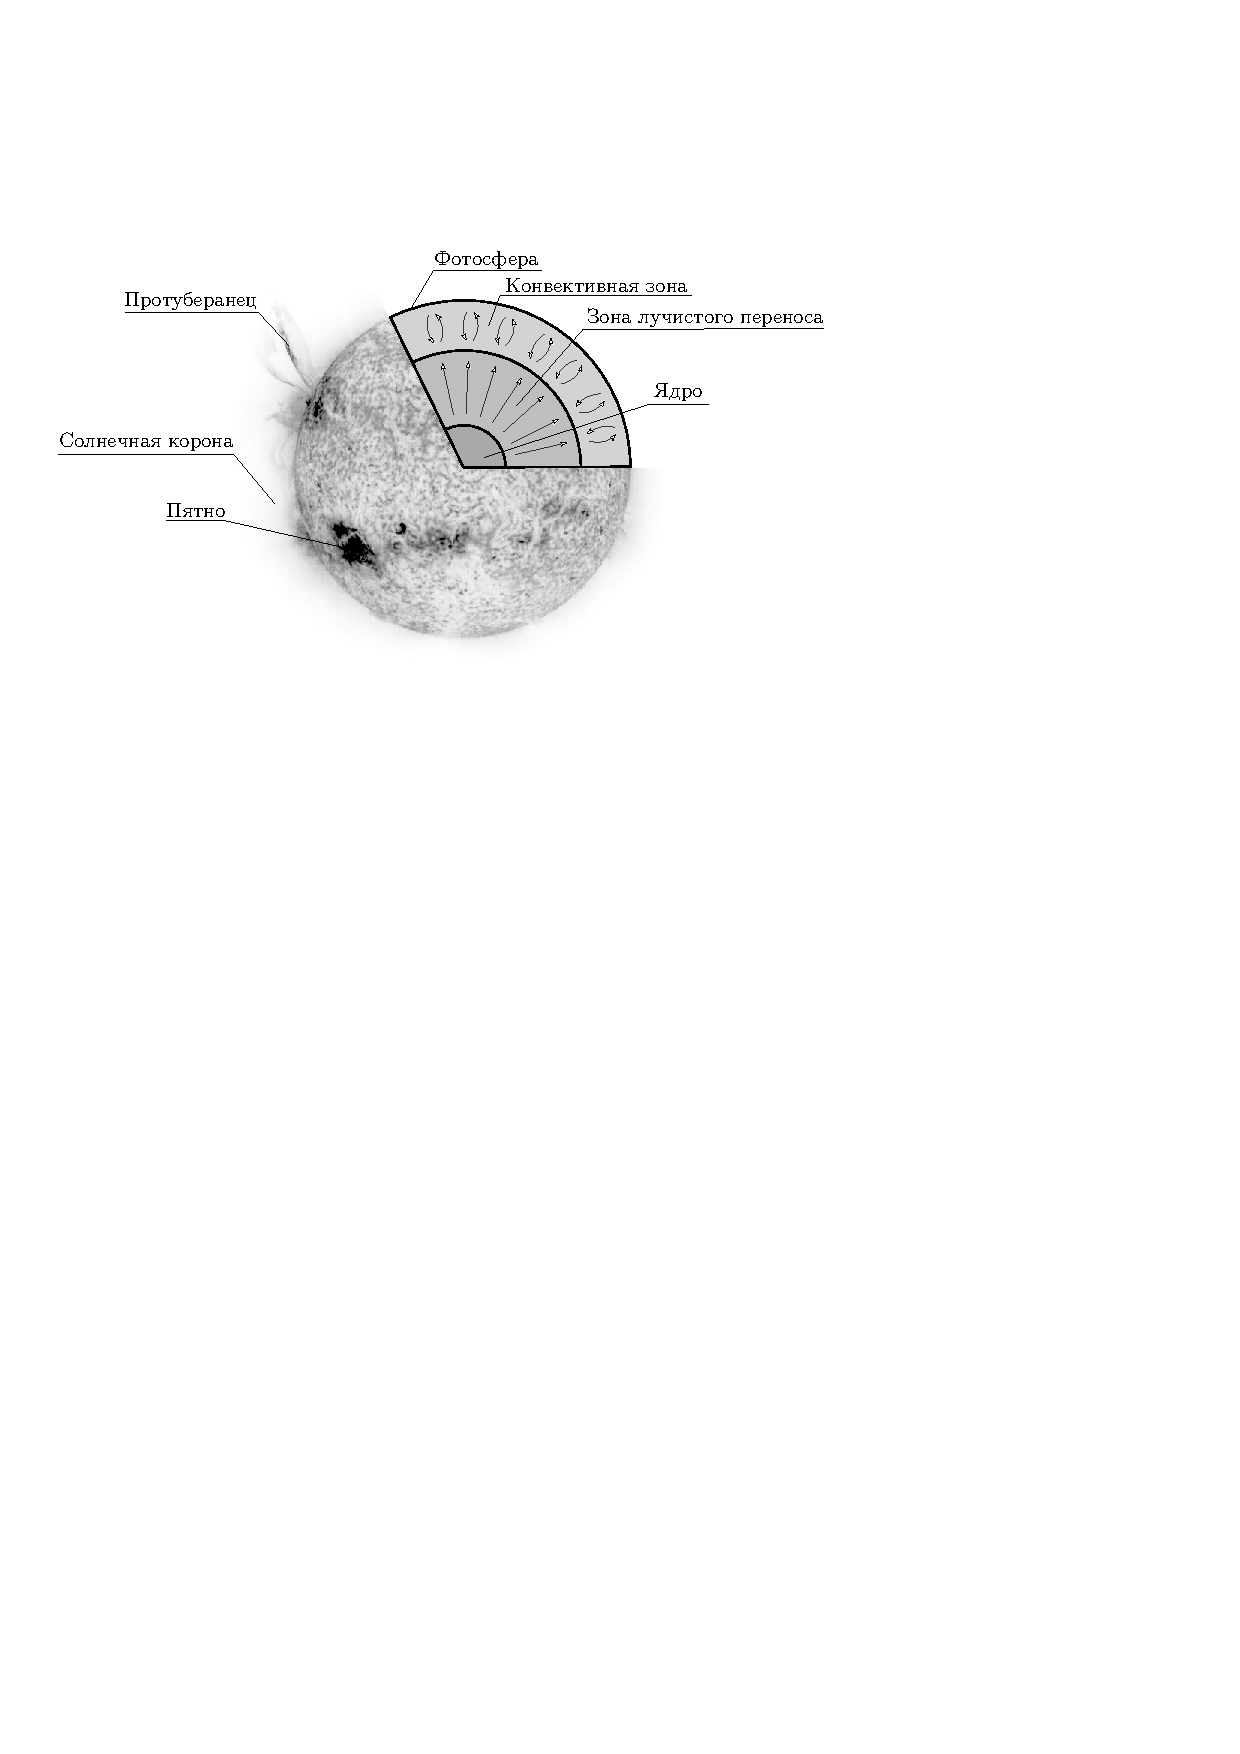
\includegraphics[width=0.65\textwidth]{sun}
\caption{Строение Солнца}
\end{center}
\end{figure}

Солнце вращается не твёрдотельно --- угловая скорость на разных широтах разная, при удалении от экватора она уменьшается. Период обращения Солнца на разных широтах можно найти, наблюдая за солнечными пятнами и другими образованиями. На экваторе период вращения состовляет 25.05 суток, к полюсу он увеличивается до 34 суток. По наблюдениям за пятнами в течение длительного периода при помощи метода наименьших квадратов можно найти зависимость углового перемещения пятна за сутки от гелиографической широты:
\begin{equation}
\Delta\lambda=14.37^{\circ}-2.7^{\circ}\sin^2\varphi,
\end{equation}
где $\Delta\lambda$ --- угловое перемещение пятна, $\varphi$ --- гелиографическая широта.

Вышеприведённая формула верна только для не очень больших значений широт ($\varphi<40^{\circ}$).